\documentclass[12pt]{article}

\usepackage{times}
\usepackage[final]{graphicx}
\usepackage{hyperref}
\usepackage{verbatim}
\usepackage{enumerate}
\usepackage{color}

\setlength{\topmargin}{-0.5in}
\setlength{\oddsidemargin}{0in}
\setlength{\evensidemargin}{0in}
\setlength{\textwidth}{6.5in}
\setlength{\textheight}{9.0in}

\begin{document}

\centerline{\bf \Large CS295/CS395/CSYS395: \href{CS295_395_Syllabus.pdf}{\underline{Evolutionary Robotics}}}

\vspace{0.5cm}

\centerline{\bf \large Programming Assignment 8b of 10}
\vspace{0.25cm} \centerline{\color{red}DRAFT: Port from ODE to Bullet by Shane Celis \color{black}}
\vspace{0.5cm}

\centerline{\large Assigned: Friday, October 21, 2011}

\vspace{0.5cm}

\centerline{\large Due: Friday, October 28, 2011 by midnight}

\vspace{0.5cm}

\noindent \color{red}CHANGES: Rather than changing the way a body part is colored, I have the student draw another shape because that was easier to do with this codebase.  The contact handling function requires a little massaging to get right for C++ in Step 10.  I've taken the approach of if a step is about C++ proper, give the student an explicit step by step approach.  \color{black}

\noindent \textbf{Description:} In this week's assignment you will add sensors to your robot. You will add one binary touch sensor in each of the four lower legs: the sensor will fire when that leg is touching the ground, and will not fire when the leg is off the ground. Adding touch sensors requires four basic steps:

\begin{enumerate}

\item Set all touch sensor values to zero at the outset of each time step of the simulation.

\item Add code so that, when nearCallback is called because there is a collision between a leg and the ground plane, Bullet knows which leg collided.

\item Set the touch for that leg to 1.

\item For those legs touching the ground, draw a red sphere at the contact point  (see Fig. \ref{Fig2}).
\end{enumerate}


The following instructions will realize these four steps.

\begin{enumerate}

\item Back up Assignment\_7 on a flash drive or another computer so that you can always return to your completed seventh assignment.

\item Copy directory Assignment\_7, which contains your submitted document and the entire Bullet folder. Rename the new directory Assignment\_8.

\item Bullet allows the user to associate a pointer with each Bullet body using the method \\ \texttt{setUserPointer(void *data)}. You will create such a data structure, and store the ID of each Bullet body there. That is, the third Bullet object will have an ID of 3. In \verb|RagdollDemo.h| below the \verb|oneStep| declaration, create an array of integers \texttt{int IDs[10]} (9 for the body parts, and 1 for the ground).

\item Just after the array is created, set the $i$th element of the array to $i$.

\item In \texttt{CreateBox(...)} and \texttt{CreateCylinder(...)}, after the Bullet body has been created, associate a pointer to the correct element in this array with the object: \\
    \texttt{body[index]->setUserPointer(\&IDs[index]);}\\
Also, associate the ground collision object \verb|fixedGround| with an ID of 9.  

\item Now, we need to setup a means of determining which objects are in contact with the ground.  There is more than one way of doing this with Bullet.  But we will do this by setting up a callback function that is called after every contact point has been processed.  Add the following function to \verb|RagdollDemo.cpp| before the \verb|initPhysics| method.

\begin{verbatim}
bool myContactProcessedCallback(btManifoldPoint& cp,
                                void* body0, void* body1)
{
  int *ID1, *ID2;
  btCollisionObject* o1 = static_cast<btCollisionObject*>(body0);
  btCollisionObject* o2 = static_cast<btCollisionObject*>(body1);
  int groundID = 9;

  ID1 = static_cast<int*>(o1->getUserPointer());
  ID2 = static_cast<int*>(o2->getUserPointer());

  /* Your code will go here. See the next step.  */

  return false;
}
\end{verbatim}  

You've defined this function, but Bullet does not know about it yet.  So, add this as the first line to the \verb|initPhysics| method: \\\verb|gContactProcessedCallback = myContactProcessedCallback;|

Recompile and run until there are no errors.  You won't see any difference yet.

\begin{figure}
\centerline{
a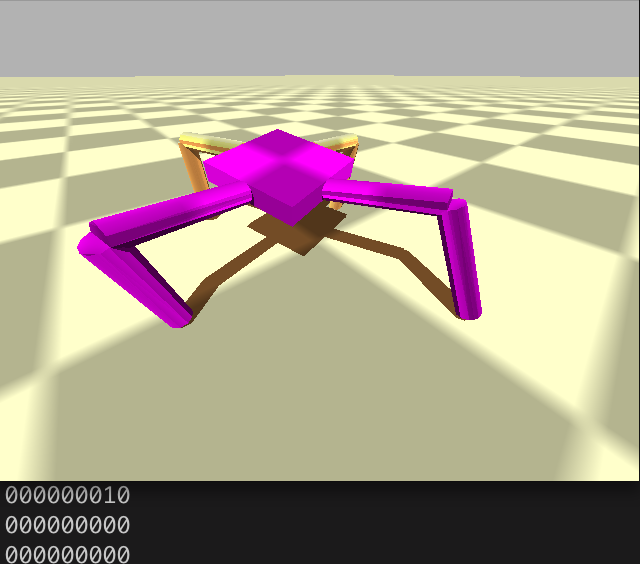
\includegraphics[height=5cm]{Fig2a}
b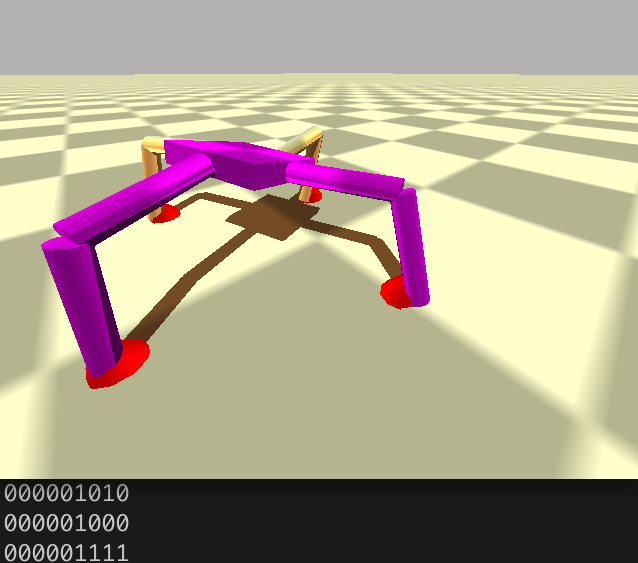
\includegraphics[height=5cm]{Fig2b}
c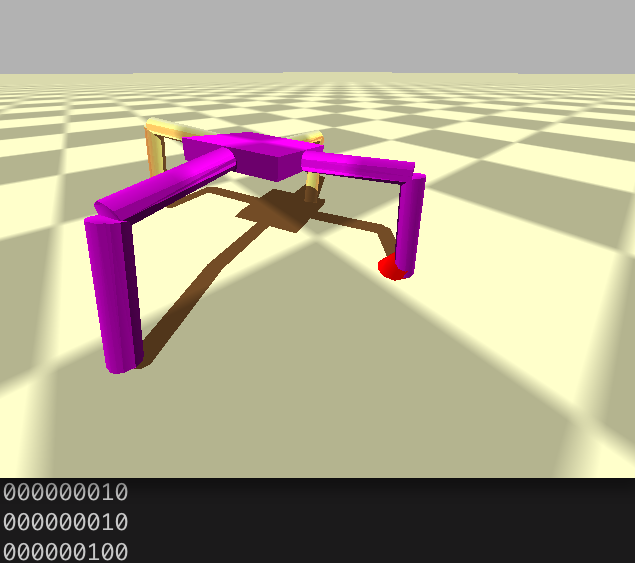
\includegraphics[height=5cm]{Fig2c}}
\caption{Visual display of the touch sensors firing: a) no sensors; b) all sensors; and c) one sensor.}
\label{Fig2} % Mislabeled.
\end{figure}

\begin{figure}
\centerline{
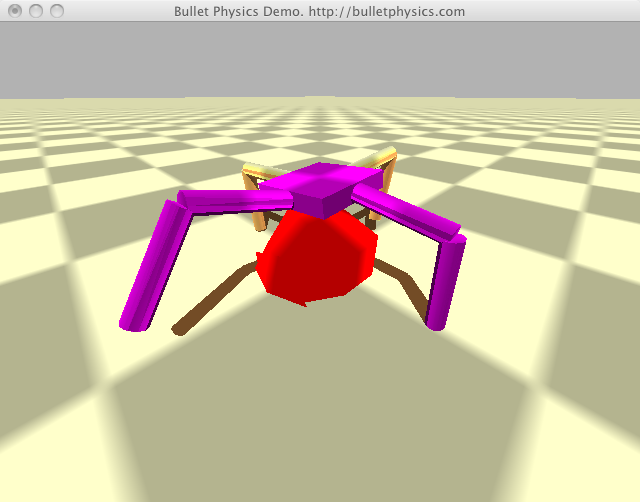
\includegraphics[height=5cm]{Fig1}}
\caption{Draw a sphere at location (0,0,0) into the scene.}
\label{Fig1}
\end{figure}


\item Once you have these IDs, print them to the output terminal:\\
  \verb|printf("ID1 = %d, ID2 = %d\n", *ID1, *ID2);|\\ Recompile and rerun. You should get something like the following when the simulation is running unpaused:
    \begin{verbatim}
ID1 = 9, ID2 = 6
ID1 = 9, ID2 = 7
ID1 = 9, ID2 = 5
ID1 = 9, ID2 = 7
\end{verbatim}
    If the robot is moving randomly (Fig. \ref{Fig2}), only the four lower legs (with IDs 5,6,7 and 8) will come into contact with the ground plane.

\item Now, in \verb|RagdollDemo.h|, create a new integer array that will store the values of the four touch sensors:\\
    \texttt{int touches[10];} \\
    \texttt{touches[i]} will be set to 1 when the touch sensor in the $i$th body part is firing, and zero otherwise. Only \texttt{touches[5]} through \texttt{touches[8]} will be used.

%\newpage

\item Calls to \verb|myContactProcessedCallback| are made when \verb|stepSimulation| is called.  So, we need to set all of the touch sensors to zero before calling \texttt{stepSimulation}, and then set all of the touch sensors that are firing to one during the \texttt{myContactProcessedCallback} calls. So before calling \texttt{stepSimulation}, add a \texttt{for} loop that sets each element of \texttt{touches} to zero.

\item In \texttt{myContactProcessedCallback}, after the print statement you can turn on the corresponding touch sensors as follows:
\begin{verbatim}
  printf("ID1 = %d, ID2 = %d\n", *ID1, *ID2);
  touches[*ID1] = 1;
  touches[*ID2] = 1;
\end{verbatim}
Unfortunately, the above code won't work because \verb|touches| is a member of the \verb|RagdollDemo| instance, and the function \verb|myContactProcessedCallback| does not know about it.  So we will fix it by doing the following things:
\begin{enumerate}
  \item Above the definition of \verb|myContactProcessedCallback| in \verb|RagdollDemo.cpp| declare a new variable:
    \begin{verbatim}
static RagdollDemo* ragdollDemo;
    \end{verbatim}
  \item Add a line of code to the \verb|initPhysics| method:
\begin{verbatim}
void RagdollDemo::initPhysics()
{
  ragdollDemo = this;
  ...
\end{verbatim}
  \item Adjust the code in \verb|myContactProcessedCallback| like so:
\begin{verbatim}
  printf("*ID1 = %d, *ID2 = %d\n", *ID1, *ID2);
  ragdollDemo->touches[*ID1] = 1;
  ragdollDemo->touches[*ID2] = 1;
\end{verbatim}
\item In \verb|RagdollDemo.h| add the line \verb|public:| before the declaration of \verb|touches|. This will allow the function \verb|myContactProcessedCallback| to see the \verb|touches| member variable.
\end{enumerate}
Recompile and rerun.  Your touch sensors might be working, but you can't see them yet.

\item Somewhere within the \\
    \texttt{if ( !pause ) \{}\\
    clause of the method \texttt{clientMoveAndDisplay} create a \texttt{for} loop that prints out the values of \texttt{touches}. When the simulation is run it should produce something like: \\
    \texttt{00001101}\\
    \texttt{00000101}\\
    \texttt{...}\\
    \texttt{00001000}\\
    (You can see this in Fig. \ref{Fig2}).

\item Now we want to see these contact points visually.  One way to do this is to use the Bullet demo's built-in key commands: hit 'c' and 'w' and the black lines show the contact normals.  However, we can do better than that.  

\item We want to add something more to the rendering.  The Bullet Demos have a \verb|renderme| method that we will use.  Add this method declaration to the \verb|RagdollDemo.h| class:
\begin{verbatim}
    virtual void renderme() {
      extern GLDebugDrawer gDebugDrawer;
      GlutDemoApplication::renderme(); /* Call the parent method. */
      /* Make a circle with a 0.9 radius at (0,0,0) with RGB color (1,0,0). */
      gDebugDrawer.drawSphere(btVector3(0.,0.,0.), 0.9, btVector3(1., 0., 0.));
    }
\end{verbatim}
You should see something like Fig. \ref{Fig1}.  Capture an image of this and copy it into your document.

\item What we want is to put little red spheres at each of our contact points.  First we need to capture the information about where those points are.  Add a new member to the \verb|RagdollDemo| class:
\begin{verbatim}
    int  touches[10];
    btVector3 touchPoints[10];
\end{verbatim}

\item Capture the points in \verb|myContactProcessedCallback| like so:
\begin{verbatim}
    ragdollDemo->touches[*ID1] = 1;
    ragdollDemo->touches[*ID2] = 1;
    ragdollDemo->touchPoints[*ID1] = cp.m_positionWorldOnB;
    ragdollDemo->touchPoints[*ID2] = cp.m_positionWorldOnB;
\end{verbatim}

\item Now, inside the \texttt{renderme} method, you can include an \texttt{if} clause that will draw a red sphere with a radius of 0.2 at the $i$th touch point if it is being touched. When you compile and run the simulation, you should see that whenever a lower leg comes in contact with the ground, a red sphere appears, and disappears when it is lifted above the ground. Capture three images showing different legs doing this as in Fig. \ref{Fig2}, copy them into your document and submit to the T.A.

\end{enumerate}

\end{document} 
